\documentclass[10pt,twocolumn,letterpaper]{article}

\usepackage{cvpr}
\usepackage{times}
\usepackage{epsfig}
\usepackage{graphicx}
\usepackage{amsmath}
\usepackage{amssymb}
\usepackage{multirow}
\usepackage[utf8]{inputenc}
\usepackage{stfloats}

% Include other packages here, before hyperref.

% If you comment hyperref and then uncomment it, you should delete
% egpaper.aux before re-running latex.  (Or just hit 'q' on the first latex
% run, let it finish, and you should be clear).
\usepackage[breaklinks=true,bookmarks=false]{hyperref}

\cvprfinalcopy % *** Uncomment this line for the final submission

\def\cvprPaperID{****} % *** Enter the CVPR Paper ID here
\def\httilde{\mbox{\tt\raisebox{-.5ex}{\symbol{126}}}}

% Pages are numbered in submission mode, and unnumbered in camera-ready
%\ifcvprfinal\pagestyle{empty}\fi
\setcounter{page}{4321}
\begin{document}

%%%%%%%%% TITLE
\title{MRNet with Alternate Pretrained Features}

\author{Shayne Miel\\
Stanford University\\
Stanford, CA, USA\\
{\tt\small smiel@stanford.edu}
% % For a paper whose authors are all at the same institution,
% % omit the following lines up until the closing ``}''.
% % Additional authors and addresses can be added with ``\and'',
% % just like the second author.
% % To save space, use either the email address or home page, not both
% \and
% Second Author\\
% Institution2\\
% First line of institution2 address\\
% {\tt\small secondauthor@i2.org}
}

\maketitle
%\thispagestyle{empty}

%%%%%%%%% ABSTRACT
% \begin{abstract}
%    The ABSTRACT is to be in fully-justified italicized text, at the top
%    of the left-hand column, below the author and affiliation
%    information. Use the word ``Abstract'' as the title, in 12-point
%    Times, boldface type, centered relative to the column, initially
%    capitalized. The abstract is to be in 10-point, single-spaced type.
%    Leave two blank lines after the Abstract, then begin the main text.
%    Look at previous CVPR abstracts to get a feel for style and length.
% \end{abstract}

%%%%%%%%% BODY TEXT
\section{Introduction}

Reading and interpreting MRIs is a time-consuming process. Even with trained
professionals, it is easy for a clinician to misdiagnose an injury based on
an MRI reading. Improving the automated identification of abnormalities in
knee MRIs
could help prioritize which MRIs to examine first, as well as provide better early
results for patients whose scans appear normal. Model predictions could
also provide a ``second opinion'' which would reduce the possibility of missed
abnormalities. This could represent a large cost savings for hospitals and
an increased level of care for patients.

\section{Problem statement}

Given a set of three MRI series (axial, coronal, and sagittal) of a patient's
knee, we wish to predict the presence of injuries that will require surgery. In
particular, we wish to predict whether the knee is healthy, has a meniscal tear,
has an ACL tear, or has any other abnormality. Since these injuries can co-occur,
we wish to predict three independent binary values: abnormal, acl tear, and meniscus
tear.


\section{Related work}

The main purpose of this study is to replicate the results achieved by Bien, et
al's MRNet model \cite{bien2018deep}. They use a pretrained AlexNet \cite{krizhevsky2012imagenet}
model to extract features from each 2D slice of the 3D MRI volume, followed by
a global
average pooling per slice to flatten the image, and a max pooling across the
volume. Finally,
a fully connected layer and sigmoid activation are used to predict a binary
label for each series. Those three predictions (axial, coronal, and sagittal) are
then used as features in a simple logistic regression to predict the final label
in question.
This process is repeated for each of the three independent labels.

An important aspect of the MRNet model is the data augmentation done during training.
Every volume is randomly flipped horizontally, shifted horizontally by -25 to 25
pixels, and rotated by -25 to 25 degrees each time it is seen during training.
This helps prevent the model from overfitting the small data set.


\section{Technical approach}

My goals for this project are fairly simple:
\begin{enumerate}
   \item Reproduce the results obtained by Bien, et al. in \cite{bien2018deep}.
   \item Experiment with using different pretrained networks to extract features,
   specifically replacing AlexNet with GoogLeNet \cite{szegedy2015going} as Chi, et al.
   did for ultrasound images \cite{chi2017thyroid},
   ResNet \cite{he2016deep} as done in \cite{korfiatis2017residual},
   and Inception-v3 \cite{szegedy2016rethinking} as done in \cite{kim2018artificial}.
   \item If time allows, try replacing the logistic regression ensemble with
   a direct concatenation of the features from each of the three series before
   going through the fully connected layer.
\end{enumerate}

Unfortunately, while Bien, et al. did release code for the architecture of
their MRNet model, they did not release the data loading, hyperparameters, data
augmentation, ensembling, or training, or evaluation code.
This means that more of the effort for this project will be focused on simply
reproducing their results.\footnote{I wrote to the authors hoping that they
would share their code privately so that I could spend more time on enhancements,
but they said that the code is not avaialble.}

However, they did release source code for training MRNet on a set of external
validation data from the 2017 Štajduhar et al. study \cite{vstajduhar2017semi}.
This provides a good starting place for trying replicate their pipeline on
the MRNet dataset.

\section{Dataset}

The MRI data provided in the
\href{https://stanfordmlgroup.github.io/competitions/mrnet/}{MRNet challenge}
contains scans from 3 MRI types (sagittal plane T2, coronal plane T1, and axial
plane PD) with 3 labels per MRI (abnormality, ACL tear, and meniscal tear) for
1,250 examinations.


\begin{table}
\begin{center}
\begin{tabular}{|lc|c|c|c|}
\hline
Diagnosis & Label & Train & Validation & Test \\
\hline\hline
\multirow{ 3}{*}{Abnormal} & Positive & 817 & 96 & 95 \\
                           & Negative & 193 & 24 & 25 \\
                           & Total & 1010 & 120 & 120 \\
\hline
\multirow{ 3}{*}{ACL}      & Positive & 193 & 15 & 54 \\
                           & Negative & 817 & 105 & 66 \\
                           & Total & 1010 & 120 & 120 \\
\hline
\multirow{ 3}{*}{Meniscus} & Positive & 357 & 40 & 52 \\
                           & Negative & 653 & 80 & 68 \\
                           & Total & 1010 & 120 & 120 \\
\hline
\end{tabular}
\end{center}
\caption{MRNet data splits and label counts.}
\label{tab:dataset}
\end{table}


They have designated a training/validation split and have withheld the test set
for leaderboard evaluation. In order to assess the
changes I will be making, I am calling their validation set the test set, and
splitting their training set into a training and validation set. Counts of
cases and labels for each set can be seen in Table \ref{tab:dataset}.

Note that this data has already been preprocessed as described in \cite{bien2018deep}:
\begin{quotation}
\noindent
   Images were extracted from Digital Imaging and Communications in Medicine
   (DICOM) files, scaled to $256 \times 256$ pixels, and converted to Portable Network
   Graphics (PNG) format using the Python programming language (version 2.7)
   and the pydicom library (version 0.9.9).

   To account for variable pixel intensity scales within the MRI series, a
   histogram-based intensity standardization algorithm was applied to the images.
   For each series, a representative intensity distribution was learned from the
   training set exams. Then, the parameters of this distribution were used to
   adjust the pixel intensities of exams in all datasets (training, tuning, and
   validation). Under this transformation, pixels with similar values correspond
   to similar tissue types. After intensity standardization, pixel values were
   clipped between 0 and 255, the standard range for PNG images.
\end{quotation}
\section{Preliminary results}

I have been able to successfully recreate the data loading and training pipeline,
as well as the data augmentation steps, ensembling, and evaluation code.
The hyperparameters and training process are the same for every model. It is unclear
whether the current hyperparameters are the optimal ones, but the results look
promising.
Figure \ref{fig:mrnet_loss} shows the loss curves from the baseline MRNet
model for training and validation on each series and diagnosis.

The AUC values for training and validation at each
epoch can be seen in Figure \ref{fig:mrnet_auc}. The models appear to be learning
and generalizing well. The validation scores are noisy though, which is most likely
due to the extremely small data set sizes and imbalanced classes.

Table \ref{tab:results} shows the AUC on the test set as reported in
\cite{bien2018deep} and the test set (their validation set) with my reproduction
of the MRNet model. I do not have access to the test set that they used for
reporting results, so I do not expect to get exactly the same results. The AUC
is fairly close for all three diagnoses. My scores are slightly lower on
ACL and Meniscus tears, which is most likely due to the smaller data set size and
non-optimal hyperparameters.

\begin{figure*}
\begin{center}
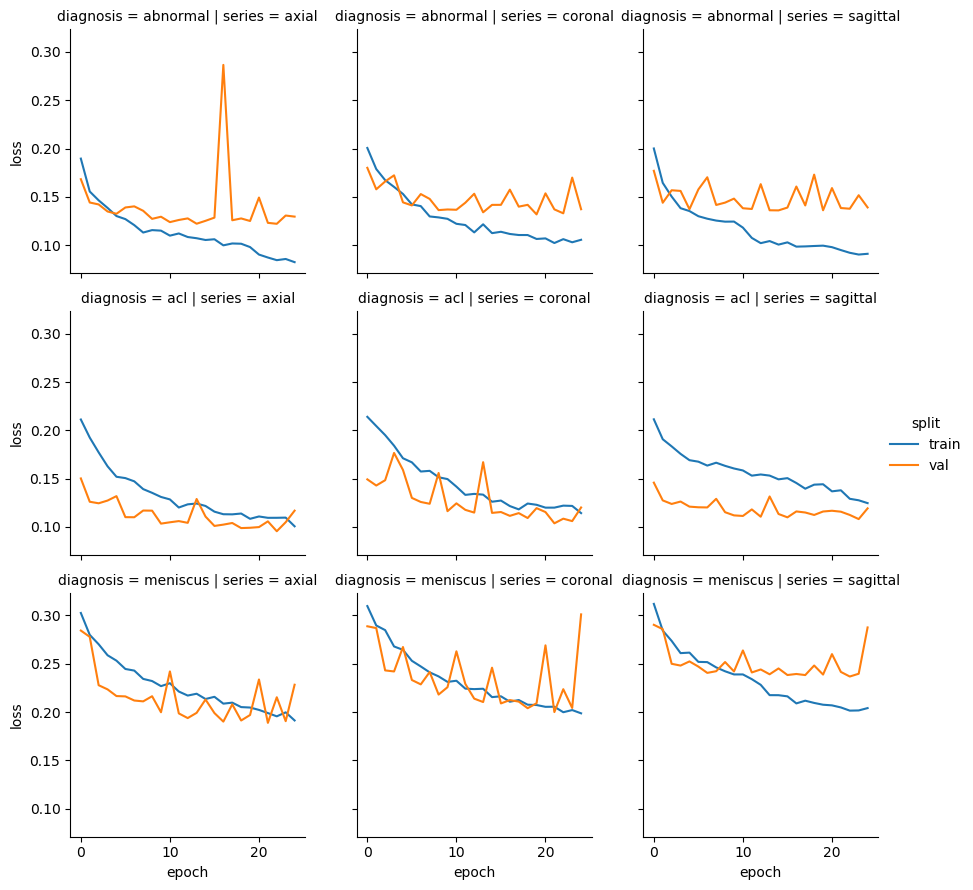
\includegraphics[width=0.5\linewidth]{../images/MRNet-aug_loss.png}
\end{center}
   \caption{Baseline loss for each diagnosis and series.}
\label{fig:mrnet_loss}
\end{figure*}

\begin{figure*}
\begin{center}
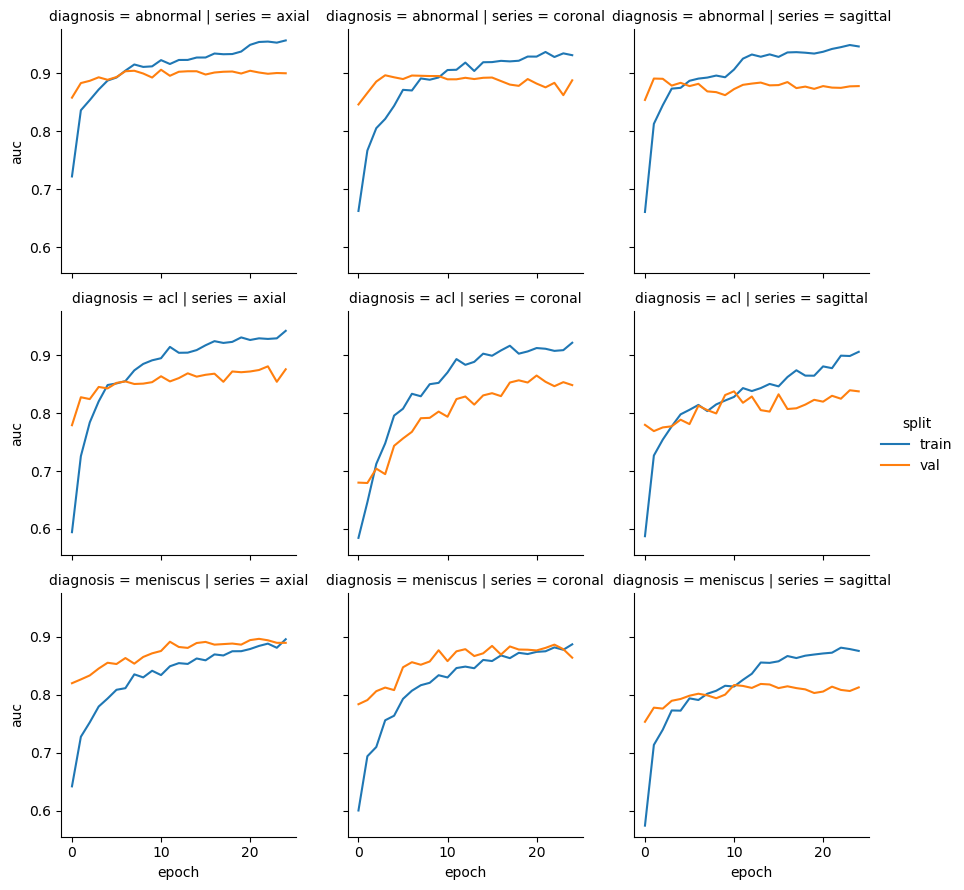
\includegraphics[width=0.5\linewidth]{../images/MRNet-aug_auc.png}
\end{center}
   \caption{Baseline AUC for each diagnosis and series.}
\label{fig:mrnet_auc}
\end{figure*}

\begin{table*}[bp]
\begin{center}
\begin{tabular}{|l|c|c|c|}
\hline
Model & Abnormal & ACL & Meniscus \\
\hline\hline
MRNet (reported) & 0.937 & 0.965 & 0.847 \\
MRNet (milestone) & 0.951 & 0.949 & 0.839 \\
\hline
\end{tabular}
\end{center}
\caption{AUC on the test set}
\label{tab:results}
\end{table*}

{\small
\bibliographystyle{ieee}
\bibliography{egbib}
}

% \begin{abstract}
%    The ABSTRACT is to be in fully-justified italicized text, at the top
%    of the left-hand column, below the author and affiliation
%    information. Use the word ``Abstract'' as the title, in 12-point
%    Times, boldface type, centered relative to the column, initially
%    capitalized. The abstract is to be in 10-point, single-spaced type.
%    Leave two blank lines after the Abstract, then begin the main text.
%    Look at previous CVPR abstracts to get a feel for style and length.
% \end{abstract}

% %%%%%%%%% BODY TEXT
% \section{Introduction}

% Please follow the steps outlined below when submitting your manuscript to
% the IEEE Computer Society Press.  This style guide now has several
% important modifications (for example, you are no longer warned against the
% use of sticky tape to attach your artwork to the paper), so all authors
% should read this new version.

% %-------------------------------------------------------------------------
% \subsection{Language}

% All manuscripts must be in English.

% \subsection{Dual submission}

% Please refer to the author guidelines on the CVPR 2017 web page for a
% discussion of the policy on dual submissions.

% \subsection{Paper length}
% Papers, excluding the references section,
% must be no longer than eight pages in length. The references section
% will not be included in the page count, and there is no limit on the
% length of the references section. For example, a paper of eight pages
% with two pages of references would have a total length of 10 pages.
% {\bf There will be no extra page charges for
%   CVPR 2017.}

% Overlength papers will simply not be reviewed.  This includes papers
% where the margins and formatting are deemed to have been significantly
% altered from those laid down by this style guide.  Note that this
% \LaTeX\ guide already sets figure captions and references in a smaller font.
% The reason such papers will not be reviewed is that there is no provision for
% supervised revisions of manuscripts.  The reviewing process cannot determine
% the suitability of the paper for presentation in eight pages if it is
% reviewed in eleven.

% %-------------------------------------------------------------------------
% \subsection{The ruler}
% The \LaTeX\ style defines a printed ruler which should be present in the
% version submitted for review.  The ruler is provided in order that
% reviewers may comment on particular lines in the paper without
% circumlocution.  If you are preparing a document using a non-\LaTeX\
% document preparation system, please arrange for an equivalent ruler to
% appear on the final output pages.  The presence or absence of the ruler
% should not change the appearance of any other content on the page.  The
% camera ready copy should not contain a ruler. (\LaTeX\ users may uncomment
% the \verb'\cvprfinalcopy' command in the document preamble.)  Reviewers:
% note that the ruler measurements do not align well with lines in the paper
% --- this turns out to be very difficult to do well when the paper contains
% many figures and equations, and, when done, looks ugly.  Just use fractional
% references (e.g.\ this line is $095.5$), although in most cases one would
% expect that the approximate location will be adequate.

% \subsection{Mathematics}

% Please number all of your sections and displayed equations.  It is
% important for readers to be able to refer to any particular equation.  Just
% because you didn't refer to it in the text doesn't mean some future reader
% might not need to refer to it.  It is cumbersome to have to use
% circumlocutions like ``the equation second from the top of page 3 column
% 1''.  (Note that the ruler will not be present in the final copy, so is not
% an alternative to equation numbers).  All authors will benefit from reading
% Mermin's description of how to write mathematics:
% \url{http://www.pamitc.org/documents/mermin.pdf}.


% \subsection{Blind review}

% Many authors misunderstand the concept of anonymizing for blind
% review.  Blind review does not mean that one must remove
% citations to one's own work---in fact it is often impossible to
% review a paper unless the previous citations are known and
% available.

% Blind review means that you do not use the words ``my'' or ``our''
% when citing previous work.  That is all.  (But see below for
% techreports.)

% Saying ``this builds on the work of Lucy Smith [1]'' does not say
% that you are Lucy Smith; it says that you are building on her
% work.  If you are Smith and Jones, do not say ``as we show in
% [7]'', say ``as Smith and Jones show in [7]'' and at the end of the
% paper, include reference 7 as you would any other cited work.

% An example of a bad paper just asking to be rejected:
% \begin{quote}
% \begin{center}
%     An analysis of the frobnicatable foo filter.
% \end{center}

%    In this paper we present a performance analysis of our
%    previous paper [1], and show it to be inferior to all
%    previously known methods.  Why the previous paper was
%    accepted without this analysis is beyond me.

%    [1] Removed for blind review
% \end{quote}


% An example of an acceptable paper:

% \begin{quote}
% \begin{center}
%      An analysis of the frobnicatable foo filter.
% \end{center}

%    In this paper we present a performance analysis of the
%    paper of Smith \etal [1], and show it to be inferior to
%    all previously known methods.  Why the previous paper
%    was accepted without this analysis is beyond me.

%    [1] Smith, L and Jones, C. ``The frobnicatable foo
%    filter, a fundamental contribution to human knowledge''.
%    Nature 381(12), 1-213.
% \end{quote}

% If you are making a submission to another conference at the same time,
% which covers similar or overlapping material, you may need to refer to that
% submission in order to explain the differences, just as you would if you
% had previously published related work.  In such cases, include the
% anonymized parallel submission~\cite{Authors14} as additional material and
% cite it as
% \begin{quote}
% [1] Authors. ``The frobnicatable foo filter'', F\&G 2014 Submission ID 324,
% Supplied as additional material {\tt fg324.pdf}.
% \end{quote}

% Finally, you may feel you need to tell the reader that more details can be
% found elsewhere, and refer them to a technical report.  For conference
% submissions, the paper must stand on its own, and not {\em require} the
% reviewer to go to a techreport for further details.  Thus, you may say in
% the body of the paper ``further details may be found
% in~\cite{Authors14b}''.  Then submit the techreport as additional material.
% Again, you may not assume the reviewers will read this material.

% Sometimes your paper is about a problem which you tested using a tool which
% is widely known to be restricted to a single institution.  For example,
% let's say it's 1969, you have solved a key problem on the Apollo lander,
% and you believe that the CVPR70 audience would like to hear about your
% solution.  The work is a development of your celebrated 1968 paper entitled
% ``Zero-g frobnication: How being the only people in the world with access to
% the Apollo lander source code makes us a wow at parties'', by Zeus \etal.

% You can handle this paper like any other.  Don't write ``We show how to
% improve our previous work [Anonymous, 1968].  This time we tested the
% algorithm on a lunar lander [name of lander removed for blind review]''.
% That would be silly, and would immediately identify the authors. Instead
% write the following:
% \begin{quotation}
% \noindent
%    We describe a system for zero-g frobnication.  This
%    system is new because it handles the following cases:
%    A, B.  Previous systems [Zeus et al. 1968] didn't
%    handle case B properly.  Ours handles it by including
%    a foo term in the bar integral.

%    ...

%    The proposed system was integrated with the Apollo
%    lunar lander, and went all the way to the moon, don't
%    you know.  It displayed the following behaviours
%    which show how well we solved cases A and B: ...
% \end{quotation}
% As you can see, the above text follows standard scientific convention,
% reads better than the first version, and does not explicitly name you as
% the authors.  A reviewer might think it likely that the new paper was
% written by Zeus \etal, but cannot make any decision based on that guess.
% He or she would have to be sure that no other authors could have been
% contracted to solve problem B.

% FAQ: Are acknowledgements OK?  No.  Leave them for the final copy.


% \begin{figure}[t]
% \begin{center}
% \fbox{\rule{0pt}{2in} \rule{0.9\linewidth}{0pt}}
%    %\includegraphics[width=0.8\linewidth]{egfigure.eps}
% \end{center}
%    \caption{Example of caption.  It is set in Roman so that mathematics
%    (always set in Roman: $B \sin A = A \sin B$) may be included without an
%    ugly clash.}
% \label{fig:long}
% \label{fig:onecol}
% \end{figure}

% \subsection{Miscellaneous}

% \noindent
% Compare the following:\\
% \begin{tabular}{ll}
%  \verb'$conf_a$' &  $conf_a$ \\
%  \verb'$\mathit{conf}_a$' & $\mathit{conf}_a$
% \end{tabular}\\
% See The \TeX book, p165.

% The space after \eg, meaning ``for example'', should not be a
% sentence-ending space. So \eg is correct, {\em e.g.} is not.  The provided
% \verb'\eg' macro takes care of this.

% When citing a multi-author paper, you may save space by using ``et alia'',
% shortened to ``\etal'' (not ``{\em et.\ al.}'' as ``{\em et}'' is a complete word.)
% However, use it only when there are three or more authors.  Thus, the
% following is correct: ``
%    Frobnication has been trendy lately.
%    It was introduced by Alpher~\cite{Alpher02}, and subsequently developed by
%    Alpher and Fotheringham-Smythe~\cite{Alpher03}, and Alpher \etal~\cite{Alpher04}.''

% This is incorrect: ``... subsequently developed by Alpher \etal~\cite{Alpher03} ...''
% because reference~\cite{Alpher03} has just two authors.  If you use the
% \verb'\etal' macro provided, then you need not worry about double periods
% when used at the end of a sentence as in Alpher \etal.

% For this citation style, keep multiple citations in numerical (not
% chronological) order, so prefer \cite{Alpher03,Alpher02,Authors14} to
% \cite{Alpher02,Alpher03,Authors14}.


% \begin{figure*}
% \begin{center}
% \fbox{\rule{0pt}{2in} \rule{.9\linewidth}{0pt}}
% \end{center}
%    \caption{Example of a short caption, which should be centered.}
% \label{fig:short}
% \end{figure*}

% %------------------------------------------------------------------------
% \section{Formatting your paper}

% All text must be in a two-column format. The total allowable width of the
% text area is $6\frac78$ inches (17.5 cm) wide by $8\frac78$ inches (22.54
% cm) high. Columns are to be $3\frac14$ inches (8.25 cm) wide, with a
% $\frac{5}{16}$ inch (0.8 cm) space between them. The main title (on the
% first page) should begin 1.0 inch (2.54 cm) from the top edge of the
% page. The second and following pages should begin 1.0 inch (2.54 cm) from
% the top edge. On all pages, the bottom margin should be 1-1/8 inches (2.86
% cm) from the bottom edge of the page for $8.5 \times 11$-inch paper; for A4
% paper, approximately 1-5/8 inches (4.13 cm) from the bottom edge of the
% page.

% %-------------------------------------------------------------------------
% \subsection{Margins and page numbering}

% All printed material, including text, illustrations, and charts, must be kept
% within a print area 6-7/8 inches (17.5 cm) wide by 8-7/8 inches (22.54 cm)
% high.
% Page numbers should be in footer with page numbers, centered and .75
% inches from the bottom of the page and make it start at the correct page
% number rather than the 4321 in the example.  To do this fine the line (around
% line 23)
% \begin{verbatim}
% %\ifcvprfinal\pagestyle{empty}\fi
% \setcounter{page}{4321}
% \end{verbatim}
% where the number 4321 is your assigned starting page.

% Make sure the first page is numbered by commenting out the first page being
% empty on line 46
% \begin{verbatim}
% %\thispagestyle{empty}
% \end{verbatim}


% %-------------------------------------------------------------------------
% \subsection{Type-style and fonts}

% Wherever Times is specified, Times Roman may also be used. If neither is
% available on your word processor, please use the font closest in
% appearance to Times to which you have access.

% MAIN TITLE. Center the title 1-3/8 inches (3.49 cm) from the top edge of
% the first page. The title should be in Times 14-point, boldface type.
% Capitalize the first letter of nouns, pronouns, verbs, adjectives, and
% adverbs; do not capitalize articles, coordinate conjunctions, or
% prepositions (unless the title begins with such a word). Leave two blank
% lines after the title.

% AUTHOR NAME(s) and AFFILIATION(s) are to be centered beneath the title
% and printed in Times 12-point, non-boldface type. This information is to
% be followed by two blank lines.

% The ABSTRACT and MAIN TEXT are to be in a two-column format.

% MAIN TEXT. Type main text in 10-point Times, single-spaced. Do NOT use
% double-spacing. All paragraphs should be indented 1 pica (approx. 1/6
% inch or 0.422 cm). Make sure your text is fully justified---that is,
% flush left and flush right. Please do not place any additional blank
% lines between paragraphs.

% Figure and table captions should be 9-point Roman type as in
% Figures~\ref{fig:onecol} and~\ref{fig:short}.  Short captions should be centred.

% \noindent Callouts should be 9-point Helvetica, non-boldface type.
% Initially capitalize only the first word of section titles and first-,
% second-, and third-order headings.

% FIRST-ORDER HEADINGS. (For example, {\large \bf 1. Introduction})
% should be Times 12-point boldface, initially capitalized, flush left,
% with one blank line before, and one blank line after.

% SECOND-ORDER HEADINGS. (For example, { \bf 1.1. Database elements})
% should be Times 11-point boldface, initially capitalized, flush left,
% with one blank line before, and one after. If you require a third-order
% heading (we discourage it), use 10-point Times, boldface, initially
% capitalized, flush left, preceded by one blank line, followed by a period
% and your text on the same line.

% %-------------------------------------------------------------------------
% \subsection{Footnotes}

% Please use footnotes\footnote {This is what a footnote looks like.  It
% often distracts the reader from the main flow of the argument.} sparingly.
% Indeed, try to avoid footnotes altogether and include necessary peripheral
% observations in
% the text (within parentheses, if you prefer, as in this sentence).  If you
% wish to use a footnote, place it at the bottom of the column on the page on
% which it is referenced. Use Times 8-point type, single-spaced.


% %-------------------------------------------------------------------------
% \subsection{References}

% List and number all bibliographical references in 9-point Times,
% single-spaced, at the end of your paper. When referenced in the text,
% enclose the citation number in square brackets, for
% example~\cite{Authors14}.  Where appropriate, include the name(s) of
% editors of referenced books.

% \begin{table}
% \begin{center}
% \begin{tabular}{|l|c|}
% \hline
% Method & Frobnability \\
% \hline\hline
% Theirs & Frumpy \\
% Yours & Frobbly \\
% Ours & Makes one's heart Frob\\
% \hline
% \end{tabular}
% \end{center}
% \caption{Results.   Ours is better.}
% \end{table}

% %-------------------------------------------------------------------------
% \subsection{Illustrations, graphs, and photographs}

% All graphics should be centered.  Please ensure that any point you wish to
% make is resolvable in a printed copy of the paper.  Resize fonts in figures
% to match the font in the body text, and choose line widths which render
% effectively in print.  Many readers (and reviewers), even of an electronic
% copy, will choose to print your paper in order to read it.  You cannot
% insist that they do otherwise, and therefore must not assume that they can
% zoom in to see tiny details on a graphic.

% When placing figures in \LaTeX, it's almost always best to use
% \verb+\includegraphics+, and to specify the  figure width as a multiple of
% the line width as in the example below
% {\small\begin{verbatim}
%    \usepackage[dvips]{graphicx} ...
%    \includegraphics[width=0.8\linewidth]
%                    {myfile.eps}
% \end{verbatim}
% }


% %-------------------------------------------------------------------------
% \subsection{Color}

% Please refer to the author guidelines on the CVPR 2017 web page for a discussion
% of the use of color in your document.

% %------------------------------------------------------------------------
% \section{Final copy}

% You must include your signed IEEE copyright release form when you submit
% your finished paper. We MUST have this form before your paper can be
% published in the proceedings.


% {\small
% \bibliographystyle{ieee}
% \bibliography{egbib}
% }

\end{document}
